%% ============================================================================
%%  Prezentare disertație - Beamer (pdfLaTeX, Overleaf)
%%  „Analiza, tratarea și efectul valorilor lipsă în predicția seriilor de timp
%%   cu tehnici de învățare automată" - Paul-Alin Tatar
%%
%%  Imagini: încărcați folderul `img/` în proiectul Overleaf (toate fișierele
%%  referite mai jos se află deja acolo, cu nume curate).
%%
%%  -------------------------------------------------------------------------
%%  GHID DE TIMP (țintă ~12:50). Activați notele pentru repetiții:
%%     decomentați `\setbeameroption{show notes}` din preambul.
%%   01 Titlu .................. 0:20      11 Imputare: înainte/după . 0:55
%%   02 Problema ............... 0:40      12 Tabele comparative .... 0:50
%%   03 Obiectiv + întrebare ... 0:40      13 Scheduleri LR ......... 0:40
%%   04 Contribuții ............ 0:40      14 Federat 20R/50R ....... 0:50
%%   05 Seturi de date ......... 0:35      15 Ansambluri ............ 0:50
%%   06 Pipeline metodologic ... 0:45      16 Sinteză ............... 0:55
%%   07 Strategii de imputare .. 0:50      17 Limitări .............. 0:30
%%   08 Aplicația .............. 0:30      18 Direcții viitoare ..... 0:30
%%   09 Module de experiment ... 0:35      19 Concluzie ............. 0:35
%%   10 Cele 6 experimente ..... 0:25      20 Mulțumiri / Q&A ....... 0:15
%% ============================================================================

\documentclass[aspectratio=169, 11pt]{beamer}

%% ---- Codare, limbă, fonturi -------------------------------------------------
\usepackage[T1]{fontenc}
\usepackage[utf8]{inputenc}
\usepackage[romanian]{babel}
\usepackage{lmodern}
\usepackage[sfdefault]{FiraSans} % font modern; dacă lipsește, comentați linia (rămâne lmodern)
\usepackage{textcomp}            % glife · (middot) etc.

%% ---- Grafică, tabele, casete ------------------------------------------------
\usepackage{graphicx}
\graphicspath{{img/}}
\usepackage{booktabs}
\usepackage{colortbl}
\usepackage{tikz}
\usetikzlibrary{arrows.meta, positioning}
\usepackage[most]{tcolorbox}

%% ---- Paletă de culori -------------------------------------------------------
\definecolor{primary}{HTML}{3B2E73}   % indigo profund
\definecolor{teal}{HTML}{1F8A8A}      % teal (gradient)
\definecolor{accent}{HTML}{E8625B}    % coral (accent / evidențieri)
\definecolor{good}{HTML}{2E9E6B}      % verde (rezultate bune)
\definecolor{bad}{HTML}{D7484B}       % roșu (rezultate slabe)
\definecolor{ink}{HTML}{222222}

%% ---- Stil beamer ------------------------------------------------------------
\usetheme{default}
\setbeamertemplate{navigation symbols}{}
\setbeamercolor{normal text}{fg=ink}
\setbeamercolor{structure}{fg=primary}
\setbeamercolor{frametitle}{bg=primary, fg=white}
\setbeamercolor{title}{fg=white}
\setbeamercolor{author in head/foot}{bg=primary, fg=white}
\setbeamerfont{frametitle}{series=\bfseries, size=\large}
\setbeamertemplate{itemize item}{\color{accent}\small$\blacktriangleright$}
\setbeamertemplate{itemize subitem}{\color{teal}\footnotesize$\bullet$}
\setbeamertemplate{itemize subsubitem}{\color{teal}\footnotesize$\cdot$}

% Titlu de cadru cu bară de accent
\setbeamertemplate{frametitle}{%
  \nointerlineskip%
  \begin{beamercolorbox}[wd=\paperwidth, ht=3.0ex, dp=1.3ex, leftskip=.45cm, rightskip=.45cm]{frametitle}%
    \usebeamerfont{frametitle}\insertframetitle%
  \end{beamercolorbox}%
  \vskip-0.4pt\hbox{\color{accent}\rule{\paperwidth}{1.6pt}}%
}

% Subsol cu autor + numărul cadrului
\setbeamertemplate{footline}{%
  \leavevmode%
  \hbox{%
    \begin{beamercolorbox}[wd=.6\paperwidth, ht=2.6ex, dp=1.1ex, leftskip=.45cm]{author in head/foot}%
      \footnotesize Paul-Alin Tatar%
    \end{beamercolorbox}%
    \begin{beamercolorbox}[wd=.4\paperwidth, ht=2.6ex, dp=1.1ex, rightskip=.45cm]{author in head/foot}%
      \hfill\footnotesize\insertframenumber\,/\,\inserttotalframenumber%
    \end{beamercolorbox}%
  }%
}

%% ---- Casete reutilizabile ---------------------------------------------------
\newtcolorbox{keybox}{colback=accent!10, colframe=accent, boxrule=1pt, arc=4pt,
  left=7pt, right=7pt, top=4pt, bottom=4pt}
\newtcolorbox{card}{colback=primary!6, colframe=primary!55, boxrule=0.8pt, arc=4pt,
  left=6pt, right=6pt, top=5pt, bottom=5pt}
\newtcbox{\goodpill}{nobeforeafter, box align=base, colback=good!12, colframe=good,
  arc=3pt, boxrule=0.8pt, left=4pt, right=4pt, top=2pt, bottom=2pt}
\newtcbox{\badpill}{nobeforeafter, box align=base, colback=bad!12, colframe=bad,
  arc=3pt, boxrule=0.8pt, left=4pt, right=4pt, top=2pt, bottom=2pt}

% Fundal cu gradient pentru cadrele „plain" (titlu + separatoare)
\newcommand{\gradientbg}{%
  
\begin{tikzpicture}[remember picture, overlay]
    \shade[top color=primary, bottom color=teal!85]
      (current page.south west) rectangle (current page.north east);
  \end{tikzpicture}%
}

%% ---- Separatoare de secțiune -----------------------------------------------
\AtBeginSection[]{%
  \begin{frame}[plain]
    \gradientbg
    \vfill
    \centering
    {\color{white}\usebeamerfont{frametitle}\Huge\bfseries \insertsectionhead}\\[0.5em]
    {\color{accent}\rule{4cm}{2.2pt}}
    \vfill
  \end{frame}
}

%% ---- Metadate ---------------------------------------------------------------
\title[Valori lipsă în predicția seriilor de timp]{Analiza, tratarea și efectul valorilor lipsă în predicția seriilor de timp cu tehnici de învățare automată}
\author{Paul-Alin Tatar}
\date{\today}

% Pentru repetiții cu note, decomentați:
% \setbeameroption{show notes}

\begin{document}

%% ===================== 01 · TITLU ==========================================
\begin{frame}[plain]
  \gradientbg
  \centering
  \vspace*{0.5cm}
  {\color{white}\bfseries\small
    UNIVERSITATEA DE MEDICINĂ, FARMACIE, ȘTIINȚE ȘI\\
    TEHNOLOGIE „GEORGE EMIL PALADE” DIN TÂRGU MUREȘ\\[0.4em]
    FACULTATEA DE INGINERIE ȘI TEHNOLOGIA INFORMAȚIEI\\[0.3em]
    Programul de studii: INTELIGENȚĂ ARTIFICIALĂ\par}
  \vfill
  {\color{white}\bfseries\Large LUCRARE DE DISERTAȚIE\par}
  \vspace{0.4em}
  {\color{accent}\rule{5cm}{2pt}}\\[0.6em]
  \begin{minipage}{0.86\textwidth}\centering
    {\color{white}\large\bfseries Analiza, tratarea și efectul valorilor lipsă în predicția seriilor de timp cu tehnici de învățare automată.\par}
  \end{minipage}
  \vfill
  \begin{minipage}[t]{0.48\textwidth}\raggedright
    {\color{white!80}Student:}\\[0.3em]{\color{white}\bfseries Paul-Alin Tatar}
  \end{minipage}\hfill
  \begin{minipage}[t]{0.48\textwidth}\raggedleft
    {\color{white!80}Coordonator științific:}\\[0.3em]{\color{white}\bfseries Lector Univ. Dr. Roland Bolboacă}
  \end{minipage}
  \vfill
  {\color{white!80} Iulie 2026\par}
  \vspace*{0.5cm}
\end{frame}
\note{Bună ziua. Mă numesc Paul-Alin Tatar și prezint lucrarea de disertație despre efectul valorilor lipsă asupra predicției seriilor de timp. Mulțumesc coordonatorului. Întrebarea de bază: când datele au goluri, cât de mult contează felul în care le completăm?}

%% ===================== Secțiunea 1 =========================================
\section{Motivație și obiective}

%% ----- 02 · PROBLEMA -------------------------------------------------------
\begin{frame}{Problema: valorile lipsă în seriile de timp}
  \begin{columns}[T]
    \begin{column}{0.56\textwidth}
      \begin{itemize}
        \item Lipsurile apar frecvent: erori de măsurare, senzori defecți, întreruperi, pierderi la transmisie.
        \item În seriile de timp, golurile rup \textbf{dependențele temporale}, nu doar distribuția datelor.
        \item Etapa de completare (imputare) se face \textbf{înainte} de antrenare și se propagă în toate predicțiile.
      \end{itemize}
    \end{column}
    \begin{column}{0.44\textwidth}
      \begin{keybox}
        \small O imputare slabă poate crea \textbf{tendințe artificiale} și platouri care induc în eroare modelul recurent.
      \end{keybox}
    \end{column}
  \end{columns}
  \vfill
  \centering
  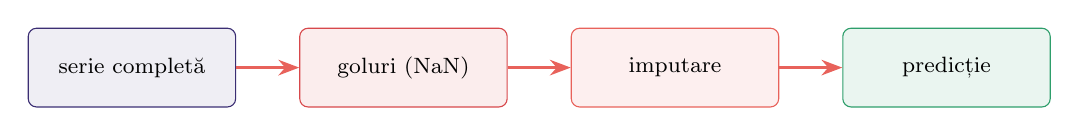
\begin{tikzpicture}[every node/.style={font=\footnotesize}]
    \node[draw=primary, fill=primary!8, rounded corners=3pt, minimum height=1cm, text width=2.4cm, align=center] (a) {serie completă};
    \node[draw=bad, fill=bad!10, rounded corners=3pt, minimum height=1cm, text width=2.4cm, align=center, right=0.8cm of a] (b) {goluri (NaN)};
    \node[draw=accent, fill=accent!10, rounded corners=3pt, minimum height=1cm, text width=2.4cm, align=center, right=0.8cm of b] (c) {imputare};
    \node[draw=good, fill=good!10, rounded corners=3pt, minimum height=1cm, text width=2.4cm, align=center, right=0.8cm of c] (d) {predicție};
    \draw[-{Stealth}, line width=1pt, accent] (a)--(b);
    \draw[-{Stealth}, line width=1pt, accent] (b)--(c);
    \draw[-{Stealth}, line width=1pt, accent] (c)--(d);
  \end{tikzpicture}
\end{frame}
\note{Valorile lipsă sunt o problemă metodologică frecventă. Spre deosebire de datele tabulare, în seriile de timp golul rupe lanțul temporal pe care modelul îl folosește. Felul în care completăm golul intră direct în antrenare, deci o imputare greșită contaminează predicțiile.}

%% ----- 03 · OBIECTIV + ÎNTREBARE -------------------------------------------
\begin{frame}{Obiectiv și întrebarea de cercetare}
  \begin{itemize}
    \item \textbf{Obiectiv:} măsurarea efectului strategiei de imputare asupra predicției cu rețele recurente (RNN, LSTM, GRU).
    \item \textbf{Abordare:} același cadru, aceleași date, aceiași hiperparametri — variem doar \textit{strategia de imputare} și \textit{arhitectura}.
  \end{itemize}
  \vfill
  \begin{keybox}
    \centering\large
    Ce contează mai mult pentru acuratețe:\\
    \textbf{arhitectura modelului} sau \textbf{calitatea imputării}?
  \end{keybox}
  \vfill
  \centering\footnotesize\color{primary}
  Două seturi de date cu dinamici diferite \textbf{·} mecanism MCAR cu seed fix \textbf{·} metrici MSE / MAE / RMSE / MAPE
\end{frame}
\note{Obiectivul este izolarea efectului imputării. Ținem totul fix și variem doar strategia de imputare și arhitectura. Întrebarea-fir-roșu al lucrării: arhitectura sau calitatea datelor de intrare? Răspunsul, anticipat, este calitatea imputării.}

%% ===================== Secțiunea 2 =========================================
\section{Cadru experimental și metodologie}

%% ----- 04 · CONTRIBUȚII ----------------------------------------------------
\begin{frame}{Contribuții proprii}
  \begin{columns}[t]
    \begin{column}{0.32\textwidth}
      \begin{card}\small\textbf{Cadru experimental unitar}\\ încărcare $\rightarrow$ MCAR $\rightarrow$ imputare $\rightarrow$ antrenare $\rightarrow$ evaluare\end{card}
    \end{column}
    \begin{column}{0.32\textwidth}
      \begin{card}\small\textbf{4 strategii de imputare}\\ ffill, fill\_mean, window\_mean, predictivă (Random Forest)\end{card}
    \end{column}
    \begin{column}{0.32\textwidth}
      \begin{card}\small\textbf{3 arhitecturi recurente}\\ RNN, LSTM, GRU în condiții identice\end{card}
    \end{column}
  \end{columns}
  \vspace{0.5em}
  \begin{columns}[t]
    \begin{column}{0.32\textwidth}
      \begin{card}\small\textbf{Învățare federată}\\ 10 utilizatori, agregare FedAvg pe mai multe runde\end{card}
    \end{column}
    \begin{column}{0.32\textwidth}
      \begin{card}\small\textbf{Ansambluri}\\ topologie paralelă și secvențială (în lanț)\end{card}
    \end{column}
    \begin{column}{0.32\textwidth}
      \begin{card}\small\textbf{Aplicație interactivă}\\ configurare, monitorizare live și export al rezultatelor\end{card}
    \end{column}
  \end{columns}
\end{frame}
\note{Contribuția principală nu e o teorie nouă, ci un cadru aplicativ unitar în care toate piesele rulează în aceeași aplicație, cu aceeași preprocesare. Asta elimină inconsistențele de comparare. Pe lângă comparația de bază, am integrat federated learning, ansambluri și o interfață interactivă.}

%% ----- 05 · SETURI DE DATE -------------------------------------------------
\begin{frame}{Două seturi de date cu dinamici diferite}
  \begin{columns}[T]
    \begin{column}{0.5\textwidth}
      \begin{card}
        \textbf{\color{primary}DSMTS}\\[0.3em]
        \small
        \begin{itemize}
          \item Sistem dinamic simulat, multivariat
          \item 4000 rânduri, 17 coloane, țintă \textit{bed1}
          \item Comportament regulat
          \item Robust chiar și la \textbf{50\%} lipsuri
        \end{itemize}
      \end{card}
    \end{column}
    \begin{column}{0.5\textwidth}
      \begin{card}
        \textbf{\color{primary}Bitcoin Historical Data}\\[0.3em]
        \small
        \begin{itemize}
          \item Date reale, volatilitate ridicată
          \item Dinamică temporală complexă
          \item Sensibil la \textit{fill\_zero} / \textit{fill\_mean}
          \item Necesită imputări mai robuste
        \end{itemize}
      \end{card}
    \end{column}
  \end{columns}
  \vfill
  \centering\footnotesize\color{primary}
  Validarea pe contexte diferite verifică dacă concluziile se mențin dincolo de un singur caz.
\end{frame}
\note{Am ales două seturi complementare. DSMTS este controlat și regulat, deci absoarbe bine artefactele de imputare. Bitcoin este volatil și expune diferențele dintre strategii. Dacă o concluzie ține pe ambele, e mai credibilă.}

%% ----- 06 · PIPELINE METODOLOGIC -------------------------------------------
\begin{frame}{Fluxul experimental}
  \centering
  \resizebox{\textwidth}{!}{%
  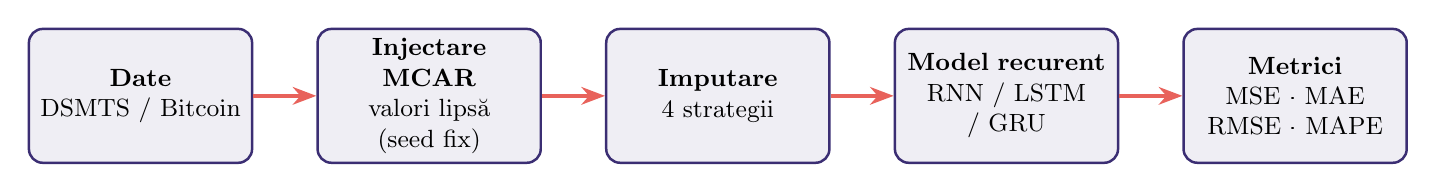
\begin{tikzpicture}[
      box/.style={rectangle, rounded corners=5pt, draw=primary, line width=0.9pt,
                  fill=primary!8, text width=2.6cm, align=center, minimum height=1.7cm,
                  font=\small},
      arr/.style={-{Stealth[length=3mm]}, line width=1.2pt, draw=accent}]
    \node[box] (d) {\textbf{Date}\\ DSMTS / Bitcoin};
    \node[box, right=0.8cm of d] (m) {\textbf{Injectare MCAR}\\ valori lipsă (seed fix)};
    \node[box, right=0.8cm of m] (i) {\textbf{Imputare}\\ 4 strategii};
    \node[box, right=0.8cm of i] (r) {\textbf{Model recurent}\\ RNN / LSTM / GRU};
    \node[box, right=0.8cm of r] (e) {\textbf{Metrici}\\ MSE · MAE\\ RMSE · MAPE};
    \draw[arr] (d)--(m);
    \draw[arr] (m)--(i);
    \draw[arr] (i)--(r);
    \draw[arr] (r)--(e);
  \end{tikzpicture}}
  \vfill
  \begin{columns}[c]
    \begin{column}{0.5\textwidth}
      \begin{card}\small \textbf{Predicție one-step-ahead:}\ $\hat{x}_{t+1}=W h_t + b$, pe ferestre fixe de lungime \textit{seq\_len}.\end{card}
    \end{column}
    \begin{column}{0.5\textwidth}
      \begin{card}\small \textbf{Împărțire cronologică} în antrenare / validare / test — fără scurgere de informație din viitor.\end{card}
    \end{column}
  \end{columns}
\end{frame}
\note{Fluxul: pornim de la date, injectăm controlat lipsuri prin MCAR cu seed fix ca să fie reproductibil, aplicăm una dintre cele patru strategii de imputare, antrenăm modelul recurent pentru predicție cu un pas înainte și evaluăm cu patru metrici. Împărțirea este cronologică, deci nu folosim viitorul în antrenare.}

%% ----- 07 · STRATEGII DE IMPUTARE ------------------------------------------
\begin{frame}{Cele patru strategii de imputare}
  \begin{columns}[T]
    \begin{column}{0.4\textwidth}
      \small
      \begin{itemize}
        \item \textbf{ffill} — propagă ultima valoare validă
        \item \textbf{fill\_mean} — media globală a coloanei
        \item \textbf{window\_mean} — media pe fereastră glisantă
        \item \textbf{predictivă} — Random Forest pe celelalte coloane
      \end{itemize}
      \vspace{0.4em}
      {\footnotesize\color{primary}(\textit{fill\_zero} este folosită ca referință; instabilă pe Bitcoin la procente mari.)}
    \end{column}
    \begin{column}{0.6\textwidth}
      \centering
      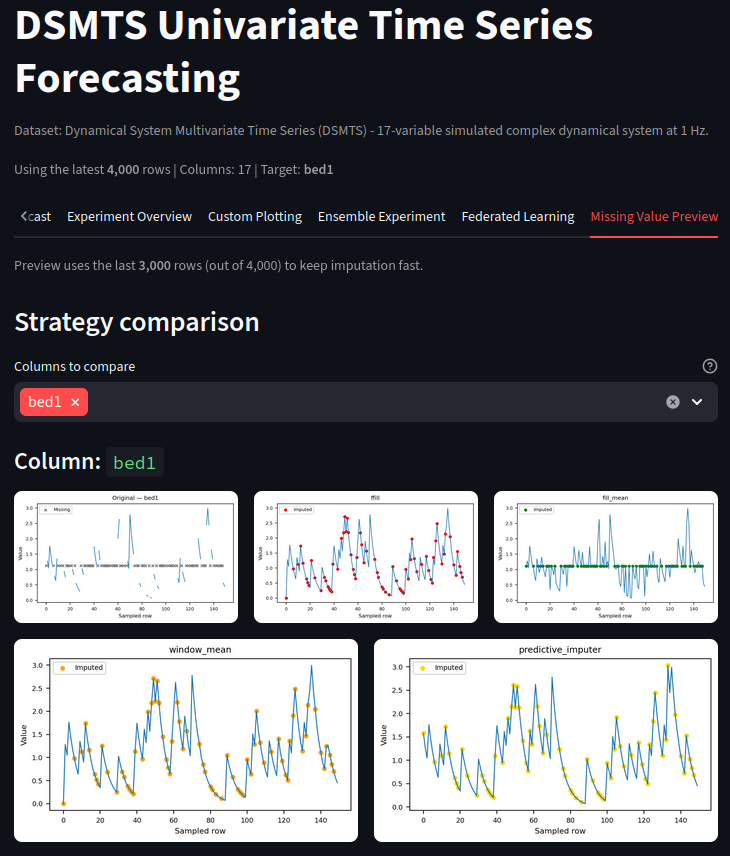
\includegraphics[width=\linewidth, height=0.72\textheight, keepaspectratio]{MissingValuePreview}\\
      {\footnotesize\color{primary} Coloana \textit{bed1}, 50\% NaN — cele cinci variante de completare.}
    \end{column}
  \end{columns}
\end{frame}
\note{Patru strategii, de la simplu la complex. Forward fill prelungește ultima valoare, deci produce platouri. Media globală ignoră poziția golului. Media pe fereastră atenuează local. Imputarea predictivă reconstruiește golul din celelalte coloane. Imaginea arată vizual cum predictiva urmărește cel mai fidel forma seriei.}

%% ----- 08 · APLICAȚIA ------------------------------------------------------
\begin{frame}{Aplicația interactivă}
  \centering
  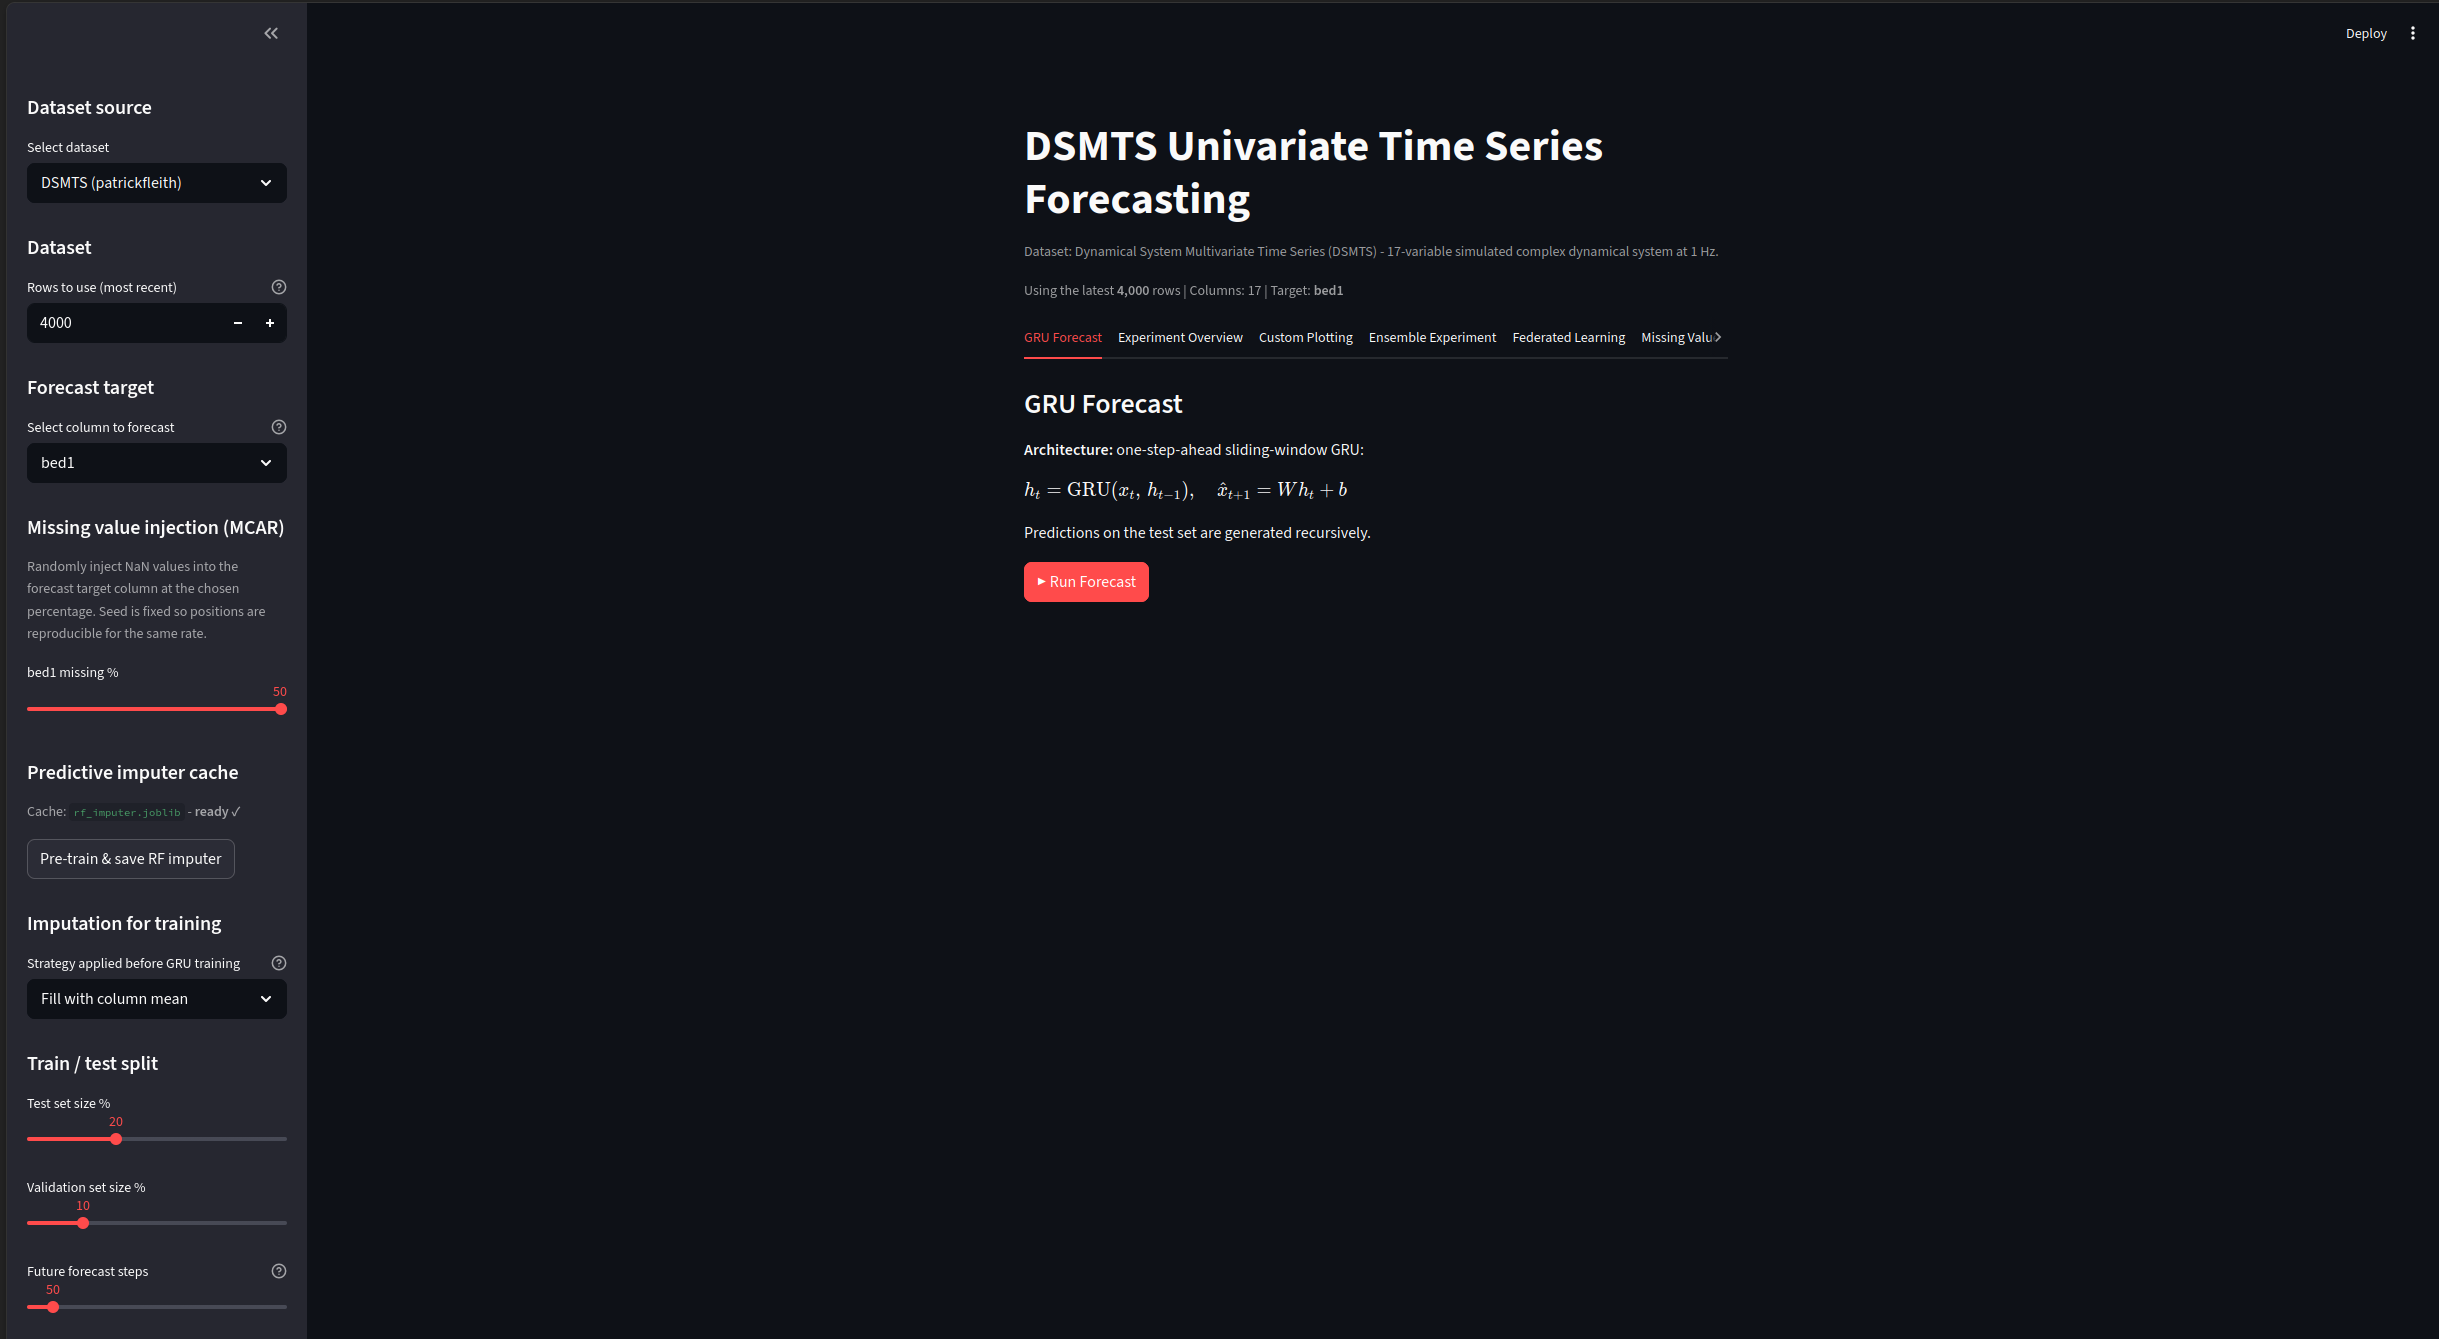
\includegraphics[width=\textwidth, height=0.78\textheight, keepaspectratio]{InterfaceFull}\\[0.2em]
  {\footnotesize\color{primary} Bară laterală pentru configurare \textbf{·} zonă centrală cu tab-uri tematice. Aceeași configurație se propagă în toate scenariile.}
\end{frame}
\note{Aplicația are o bară laterală cu toți parametrii și o zonă centrală pe tab-uri. Cheia de design: bara laterală nu se resetează între tab-uri, deci aceeași configurație merge identic în experimentul standard, federat și de ansamblu. Asta garantează comparabilitatea.}

%% ----- 09 · MODULE DE EXPERIMENT -------------------------------------------
\begin{frame}{Module de experimentare}
  \centering
  \begin{columns}[T]
    \begin{column}{0.33\textwidth}
      \centering
      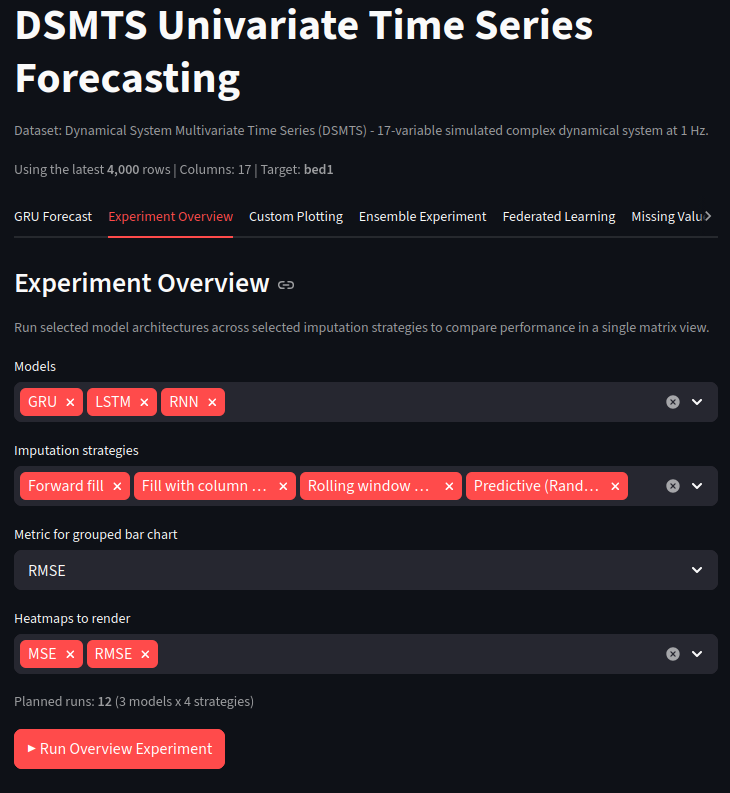
\includegraphics[width=\linewidth, height=0.66\textheight, keepaspectratio]{ExperimentOverview}\\
      {\footnotesize\color{primary} Comparare automată\\ (3 modele $\times$ 4 strategii = 12 rulări)}
    \end{column}
    \begin{column}{0.33\textwidth}
      \centering
      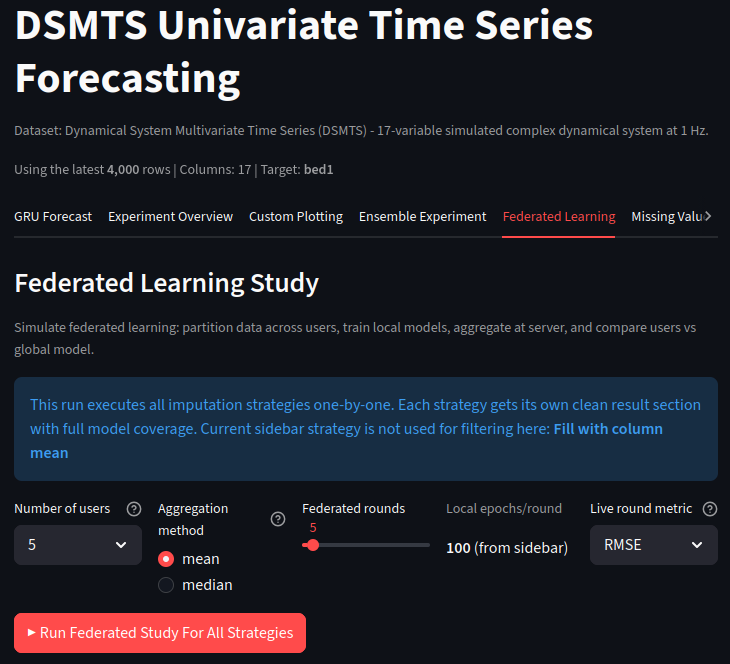
\includegraphics[width=\linewidth, height=0.66\textheight, keepaspectratio]{FederatedLearning}\\
      {\footnotesize\color{primary} Învățare federată\\ (utilizatori, runde, agregare)}
    \end{column}
    \begin{column}{0.33\textwidth}
      \centering
      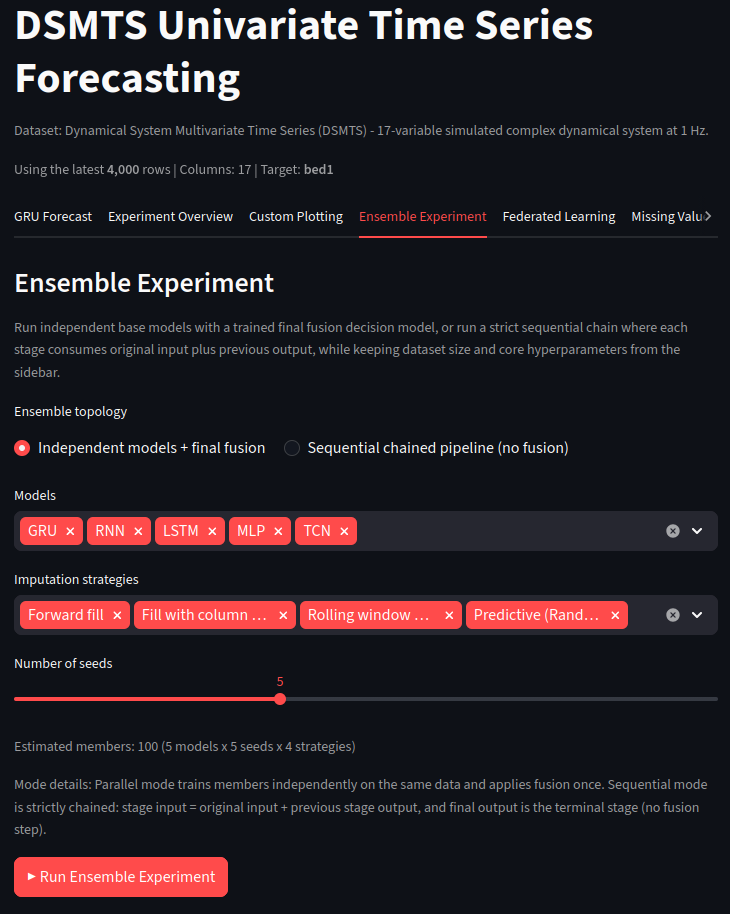
\includegraphics[width=\linewidth, height=0.66\textheight, keepaspectratio]{EnsembleExperiment}\\
      {\footnotesize\color{primary} Ansambluri\\ (paralel / secvențial)}
    \end{column}
  \end{columns}
\end{frame}
\note{Trei module cheie. Experiment Overview rulează automat toate combinațiile model-strategie și exportă CSV. Modulul federat partiționează seria pe utilizatori. Modulul de ansamblu suportă topologia paralelă și cea secvențială. Toate folosesc același cod de modelare.}

%% ----- 10 · CELE 6 EXPERIMENTE ---------------------------------------------
\begin{frame}{Cele șase experimente}
  \begin{columns}[t]
    \begin{column}{0.32\textwidth}
      \begin{card}\small\textbf{\color{accent}1.} Comparație strategii de imputare (prognoză standard)\end{card}
    \end{column}
    \begin{column}{0.32\textwidth}
      \begin{card}\small\textbf{\color{accent}2.} Scheduleri de learning rate (5 strategii)\end{card}
    \end{column}
    \begin{column}{0.32\textwidth}
      \begin{card}\small\textbf{\color{accent}3.} Federat: 10 utilizatori, 20 runde\end{card}
    \end{column}
  \end{columns}
  \vspace{0.5em}
  \begin{columns}[t]
    \begin{column}{0.32\textwidth}
      \begin{card}\small\textbf{\color{accent}4.} Federat: 10 utilizatori, 50 runde\end{card}
    \end{column}
    \begin{column}{0.32\textwidth}
      \begin{card}\small\textbf{\color{accent}5.} Ansamblu paralel (25 rulări)\end{card}
    \end{column}
    \begin{column}{0.32\textwidth}
      \begin{card}\small\textbf{\color{accent}6.} Ansamblu secvențial (5 etape)\end{card}
    \end{column}
  \end{columns}
  \vfill
  \centering\footnotesize\color{primary} Toate folosesc același protocol de evaluare pe setul de test, fără suprapunere cu antrenarea.
\end{frame}
\note{Șase experimente: comparația de imputare, schedulerii de learning rate, două scenarii federate (20 și 50 de runde), și două topologii de ansamblu. Toate cu același protocol de test. Următoarele slide-uri arată rezultatele.}

%% ===================== Secțiunea 3 =========================================
\section{Rezultate}

%% ----- 11 · IMPUTARE: ÎNAINTE / DUPĂ ---------------------------------------
\begin{frame}{Imputarea schimbă totul (GRU, DSMTS, \textit{bed1})}
  \begin{columns}[T]
    \begin{column}{0.5\textwidth}
      \centering
      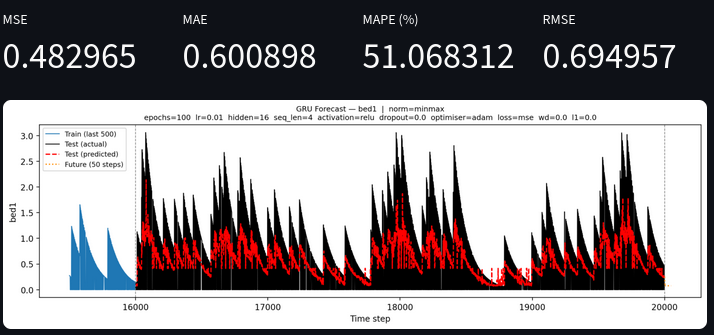
\includegraphics[width=\linewidth, height=0.5\textheight, keepaspectratio]{Fill-0}\\[0.3em]
      \badpill{\textbf{fill\_zero}}\quad \badpill{\textbf{MAPE 51.07\%}}\quad \badpill{RMSE 0.695}
    \end{column}
    \begin{column}{0.5\textwidth}
      \centering
      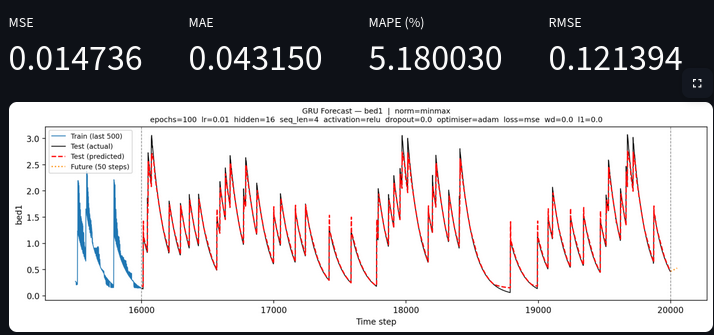
\includegraphics[width=\linewidth, height=0.5\textheight, keepaspectratio]{PredictiveInputer}\\[0.3em]
      \goodpill{\textbf{predictivă}}\quad \goodpill{\textbf{MAPE 5.18\%}}\quad \goodpill{RMSE 0.121}
    \end{column}
  \end{columns}
  \vfill
  \centering\small\color{primary}
  Aceeași configurație de model. Diferența: doar strategia de imputare. RMSE scade de \textbf{$\sim$6$\times$}.
\end{frame}
\note{Acesta e rezultatul-vedetă. Același GRU, aceiași hiperparametri, aceeași țintă. În stânga, completare cu zero: MAPE de 51\%, predicția pierde structura. În dreapta, imputare predictivă: MAPE 5\%, curbele aproape se suprapun. RMSE scade de șase ori doar schimbând imputarea.}

%% ----- 12 · TABELE COMPARATIVE ---------------------------------------------
\begin{frame}{Instabilitatea strategiei \textit{fill\_mean}}
  \centering
  \small
  \begin{tabular}{lcc}
    \toprule
    \textbf{Strategie (GRU)} & \textbf{RMSE — Rularea 1} & \textbf{RMSE — Rularea 2}\\
    \midrule
    ffill          & 44.99  & 52.97\\
    window\_mean   & 57.23  & 51.85\\
    pred. imputer  & 42.16  & 48.45\\
    \rowcolor{bad!18} fill\_mean & 191.90 & 356.93\\
    \bottomrule
  \end{tabular}
  \vfill
  \begin{columns}[c]
    \begin{column}{0.55\textwidth}
      \begin{keybox}\small
        \textit{fill\_mean} aproape se \textbf{dublează} între rulări (procent diferit de lipsuri); celelalte rămân stabile.
      \end{keybox}
    \end{column}
    \begin{column}{0.45\textwidth}
      {\footnotesize\color{primary} Media globală devine tot mai nereprezentativă pe măsură ce cresc lipsurile. LSTM și RNN urmează același tipar.}
    \end{column}
  \end{columns}
\end{frame}
\note{Tabelul condensat pentru GRU, două rulări cu procente diferite de lipsuri. Fill\_mean sare de la 192 la 357 — aproape dublu — în timp ce ffill, window\_mean și predictiva rămân stabile, sub 60. Concluzia: media globală ignoră poziția golului și se degradează cu procentul de lipsuri.}

%% ----- 13 · SCHEDULERI LR --------------------------------------------------
\begin{frame}{Scheduleri de learning rate: efect secundar}
  \centering
  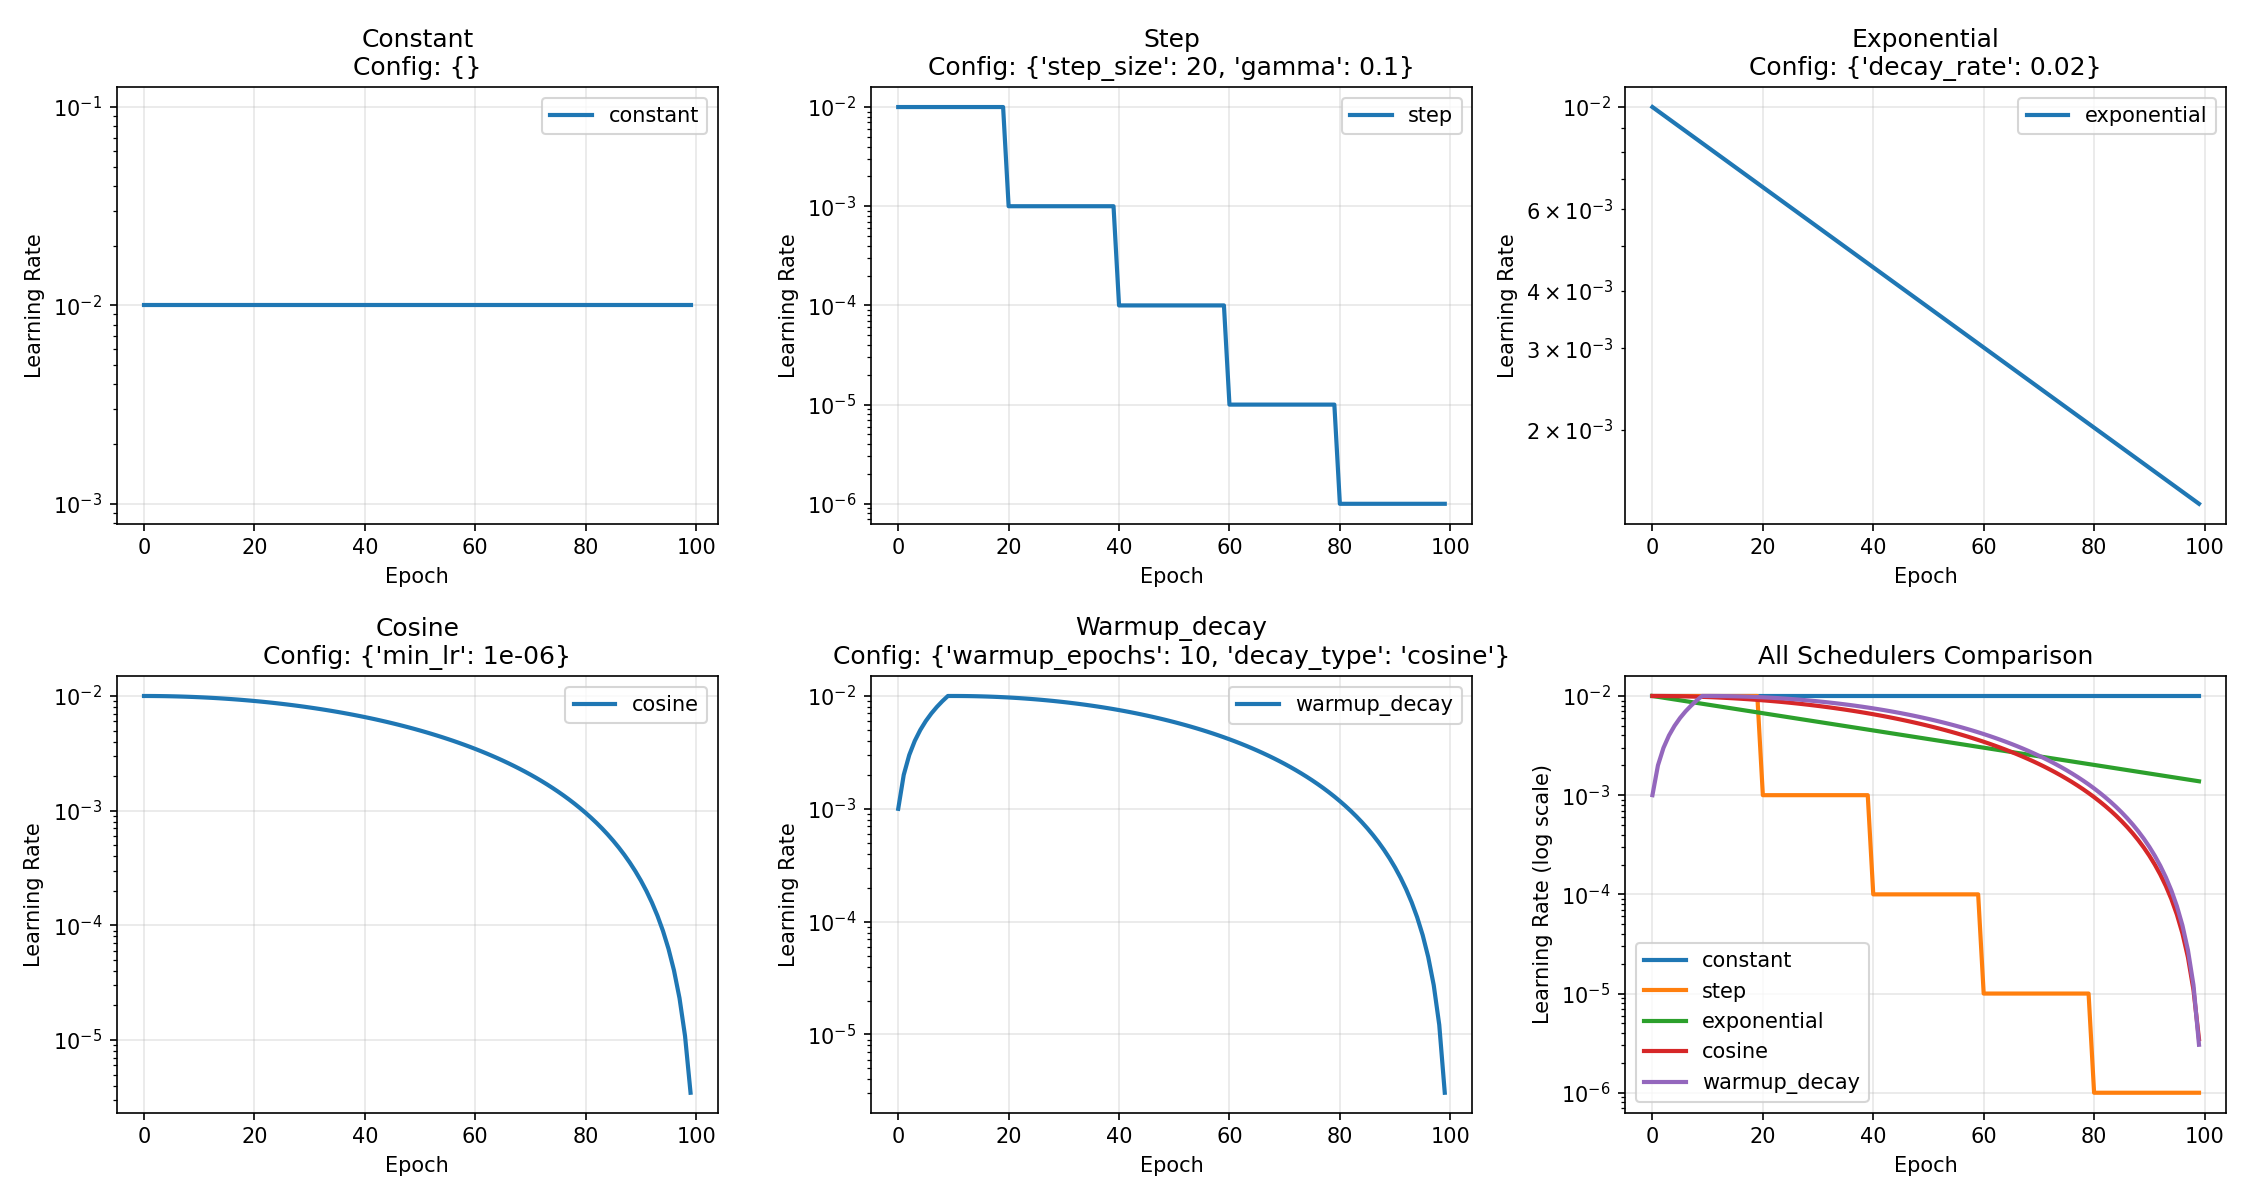
\includegraphics[width=\textwidth, height=0.42\textheight, keepaspectratio]{lr_schedulers_test}\\[0.4em]
  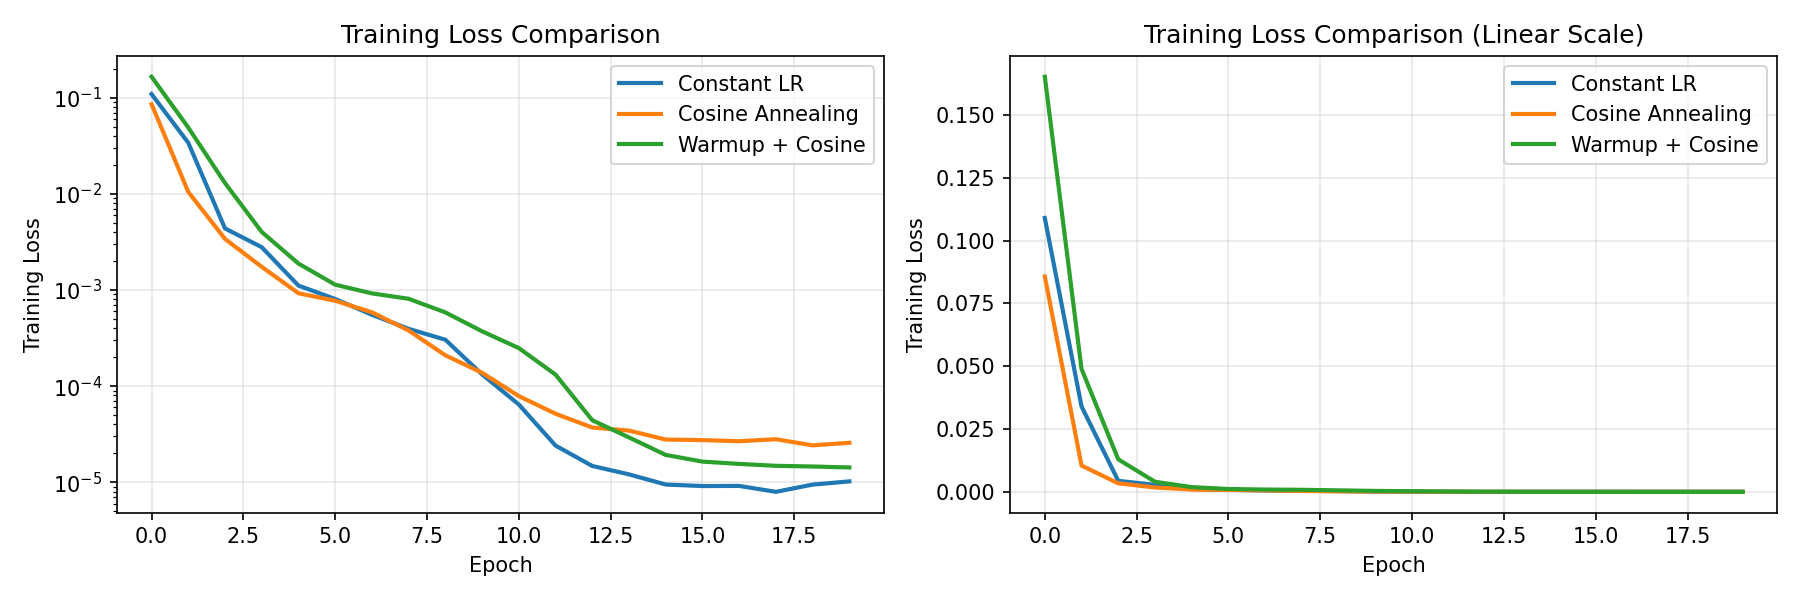
\includegraphics[width=\textwidth, height=0.30\textheight, keepaspectratio]{training_comparison}\\[0.3em]
  {\footnotesize\color{primary} Constant $\approx 10^{-5}$ vs cosine $\approx 3\times10^{-5}$ — diferență mai mică decât între oricare două strategii de imputare.}
\end{frame}
\note{Cinci scheduleri de learning rate. Toți converg rapid; diferența finală între cel mai bun și restul este de ordinul 10 la minus 5 — mult mai mică decât diferența dintre strategiile de imputare. Concluzia practică: alegi schedulerul după ce ai fixat imputarea, nu invers.}

%% ----- 14 · FEDERAT 20R / 50R ----------------------------------------------
\begin{frame}{Învățare federată: 10 utilizatori, 20 vs 50 runde}
  \centering
  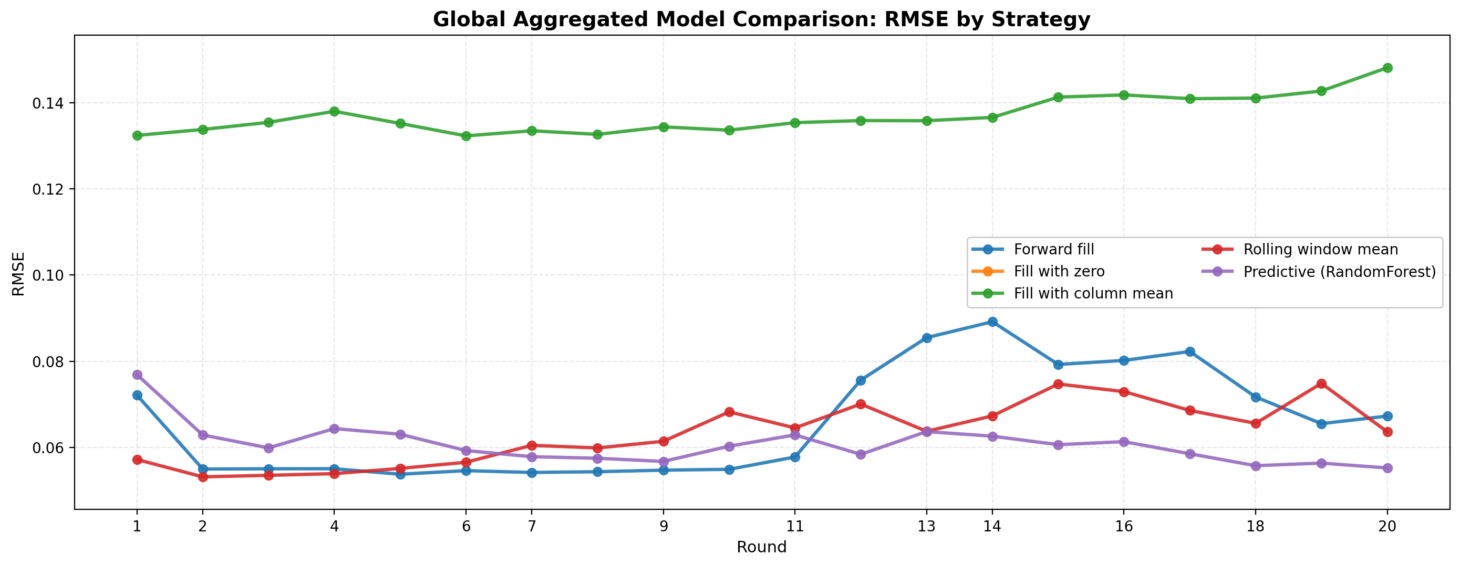
\includegraphics[width=\textwidth, height=0.33\textheight, keepaspectratio]{StrategyComparison-10U-20R}\\[0.3em]
  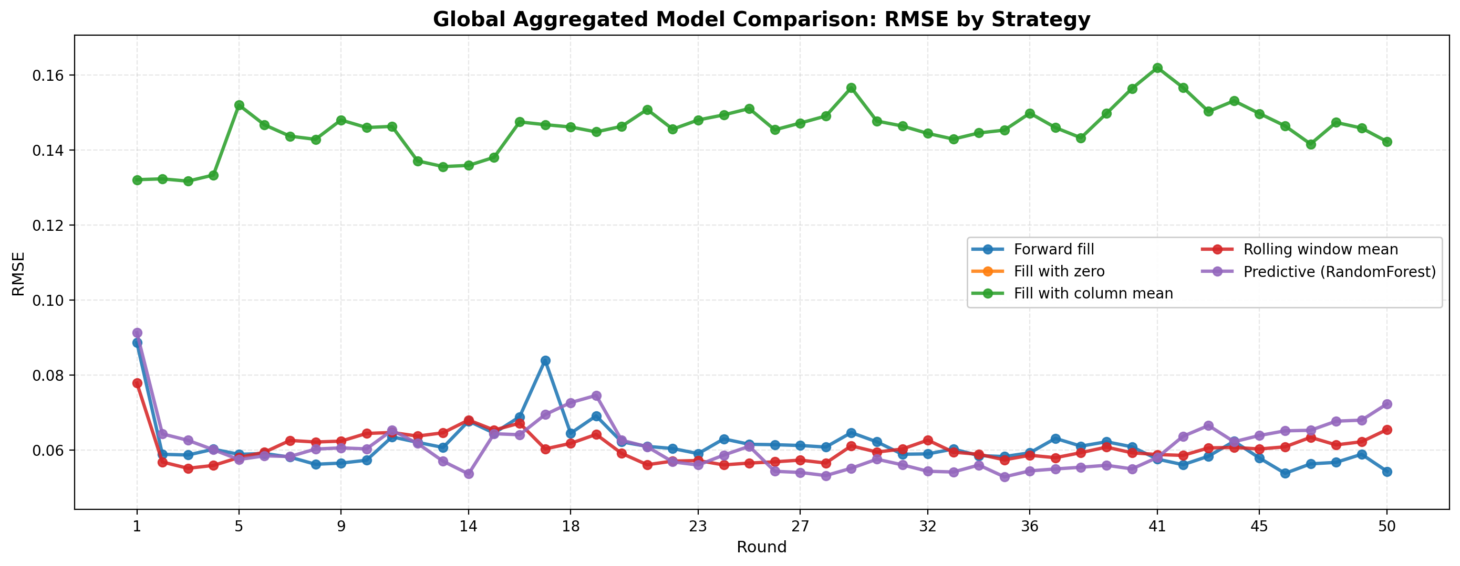
\includegraphics[width=\textwidth, height=0.33\textheight, keepaspectratio]{StrategyComparison-10U-50R}\\[0.3em]
  \begin{columns}[c]
    \begin{column}{0.5\textwidth}
      \begin{keybox}\small Convergență în \textbf{10–15 runde}; 50R nu bate 20R.\end{keybox}
    \end{column}
    \begin{column}{0.5\textwidth}
      \begin{card}\small \textit{fill\_zero} e \textbf{atenuat} aici: agregarea ponderilor = regularizare implicită.\end{card}
    \end{column}
  \end{columns}
\end{frame}
\note{Sus 20 de runde, jos 50. Fill\_mean rămâne constant cel mai slab. Celelalte converg în 3-4 runde. Important: 50 de runde nu aduc nimic peste 20 — modelul global converge devreme. Și o observație neașteptată: fill\_zero, dezastruos în standard, e atenuat aici, fiindcă agregarea modelelor locale regularizează implicit.}

%% ----- 15 · ANSAMBLURI -----------------------------------------------------
\begin{frame}{Ansambluri: paralel vs secvențial}
  \begin{columns}[T]
    \begin{column}{0.5\textwidth}
      \centering
      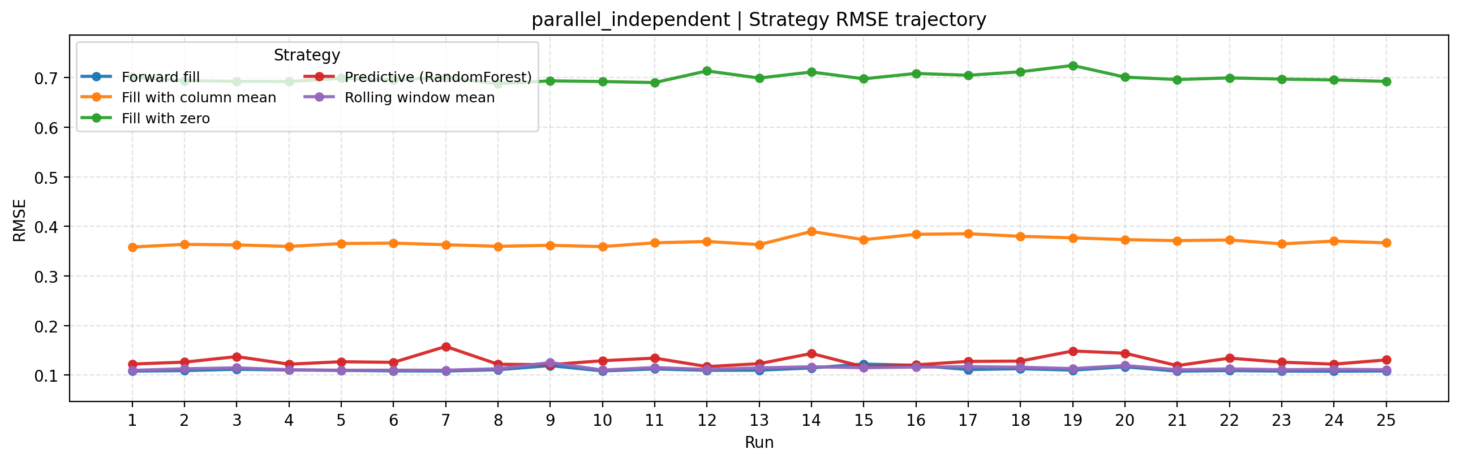
\includegraphics[width=\linewidth, height=0.34\textheight, keepaspectratio]{parallel_rmse}\\
      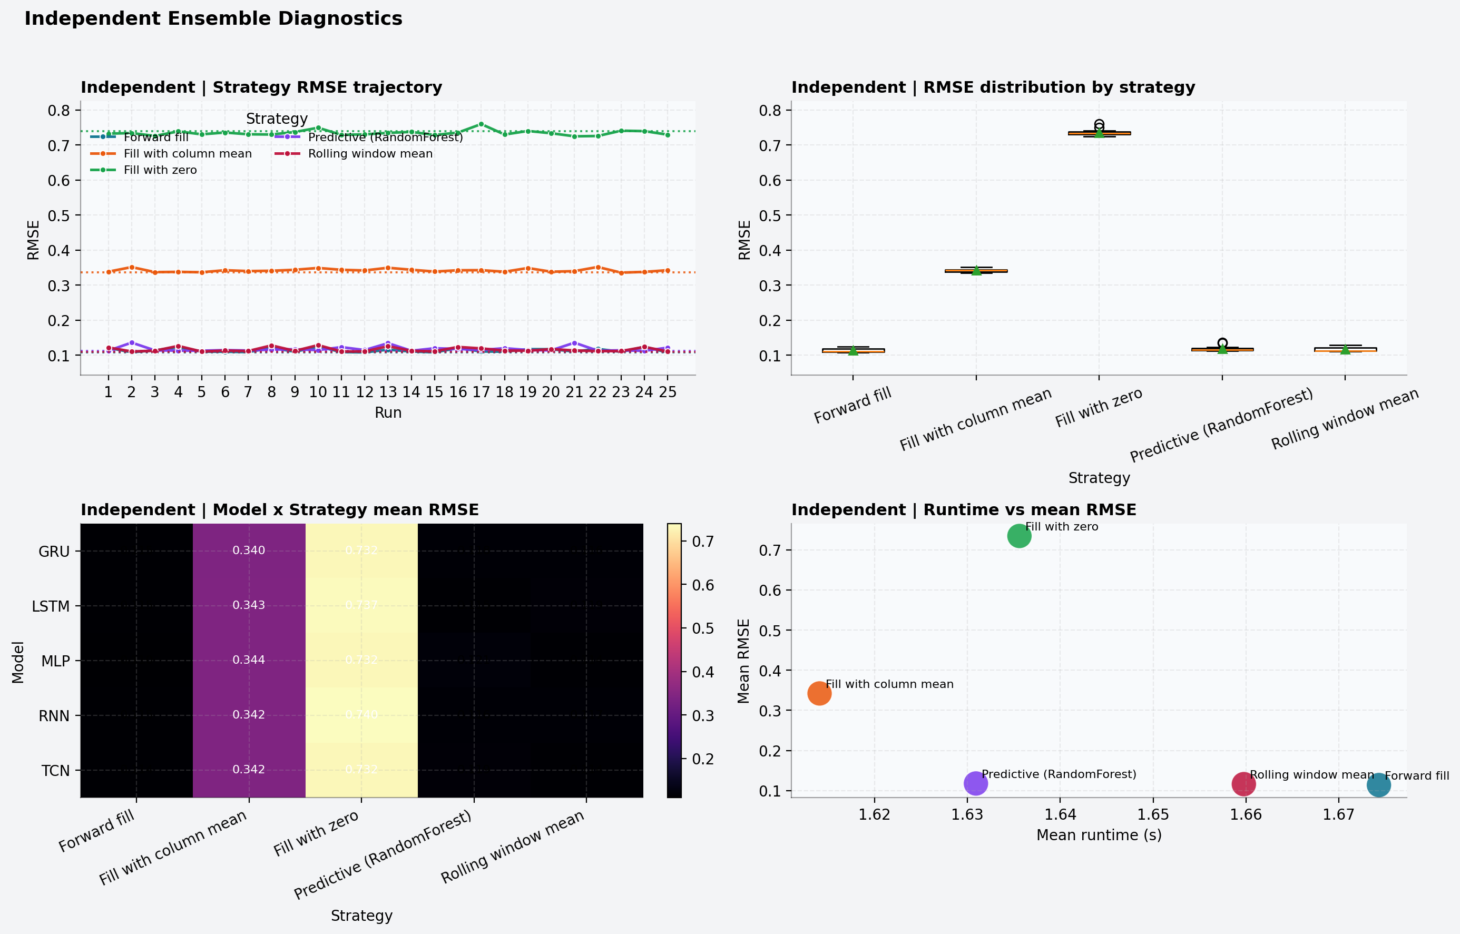
\includegraphics[width=\linewidth, height=0.30\textheight, keepaspectratio]{parallel_diagnostics}\\
      {\footnotesize\color{primary}\textbf{Paralel:} nu repară imputarea slabă\\ (fill\_mean $\approx$ 0.70, fill\_zero $\approx$ 0.35).}
    \end{column}
    \begin{column}{0.5\textwidth}
      \centering
      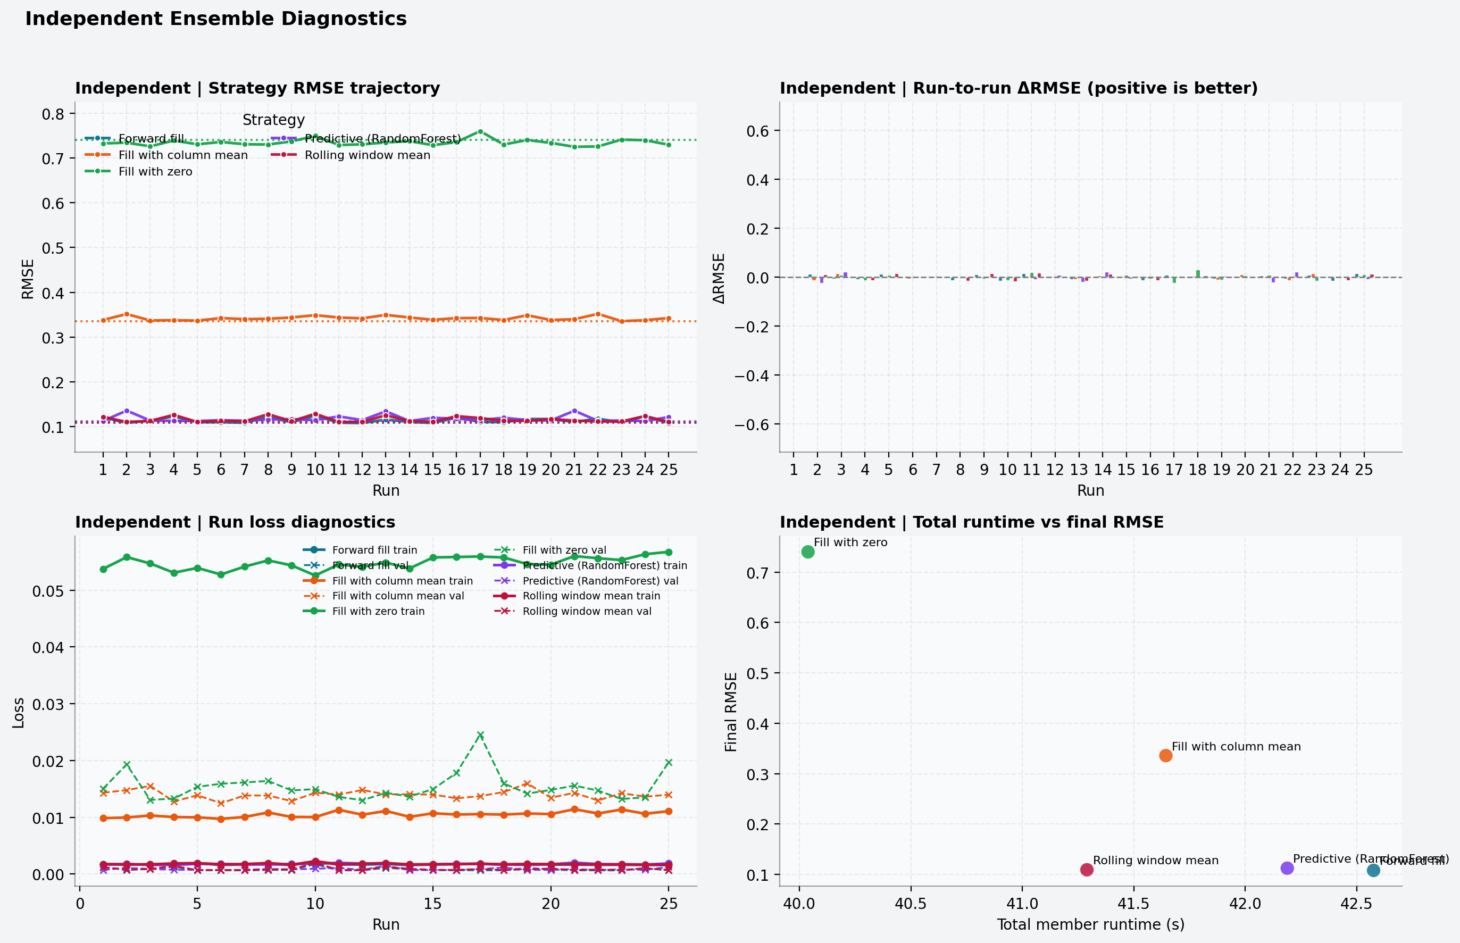
\includegraphics[width=\linewidth, height=0.5\textheight, keepaspectratio]{sequential_diagnostics}\\
      {\footnotesize\color{primary}\textbf{Secvențial:} câștig real doar până la etapa 2–3; apoi randament marginal $\approx 0$.}
    \end{column}
  \end{columns}
\end{frame}
\note{Două topologii. Paralelul mediază predicții independente: reduce varianța, dar NU corectează eroarea sistematică — dacă toate modelele văd aceleași distorsiuni, media le moștenește. De aceea fill\_mean rămâne la 0.70. Secvențialul corectează reziduuri: câștigul mare e între etapa 1 și 2, apoi se plafonează. Practic, 2-3 etape ajung.}

%% ===================== Secțiunea 4 =========================================
\section{Concluzii}

%% ----- 16 · SINTEZĂ --------------------------------------------------------
\begin{frame}{Sinteza rezultatelor}
  \begin{itemize}
    \item \textbf{Imputarea domină:} efectul ei depășește alegerea arhitecturii sau a topologiei de ansamblu.
    \item \textbf{fill\_mean} este constant cea mai slabă; \textbf{ffill} și \textbf{predictiva} sunt stabile și apropiate.
    \item \textbf{GRU și LSTM} depășesc consistent \textbf{RNN}, mai ales la imputări slabe sau lipsuri multe.
    \item \textbf{Federat:} 15–20 de runde sunt suficiente; agregarea atenuează parțial imputările proaste.
    \item \textbf{Ansamblu secvențial:} câștigul principal vine în primele 2–3 etape.
  \end{itemize}
  \vfill
  \begin{keybox}
    \centering\large \textbf{Date de intrare bune $>$ modele mai complicate.}
  \end{keybox}
\end{frame}
\note{Sinteza, în cinci puncte. Imputarea e factorul dominant. Fill\_mean cel mai slab, ffill și predictiva cele mai bune. GRU și LSTM peste RNN. În federat, 15-20 de runde ajung. În ansamblu secvențial, 2-3 etape. Mesajul: investiția în calitatea datelor bate creșterea complexității modelului.}

%% ----- 17 · LIMITĂRI -------------------------------------------------------
\begin{frame}{Limitările studiului}
  \begin{itemize}
    \item Mecanismul de lipsuri este exclusiv \textbf{MCAR}; MAR și MNAR pot da distribuții structural diferite.
    \item O singură \textbf{variabilă țintă} per set (\textit{bed1} / preț de închidere).
    \item \textbf{Hiperparametri ficși} în comparații, fără căutare sistematică per configurație.
    \item Scenariu federat \textbf{mic și omogen}: 10 utilizatori, partiții egale, consecutive.
  \end{itemize}
\end{frame}
\note{Sunt conștient de limite. Am folosit doar MCAR; mecanismele MAR și MNAR sunt mai realiste. O singură țintă per set. Hiperparametri ficși, fără tuning per configurație. Și federarea e mică și omogenă față de un sistem real.}

%% ----- 18 · DIRECȚII VIITOARE ----------------------------------------------
\begin{frame}{Direcții viitoare}
  \begin{columns}[T]
    \begin{column}{0.5\textwidth}
      \begin{card}\small\textbf{Mecanisme de lipsuri}\\ extindere la MAR și MNAR (lipsuri dependente de valori)\end{card}
      \vspace{0.5em}
      \begin{card}\small\textbf{Imputări avansate}\\ GAIN, modele generative / diffusion\end{card}
    \end{column}
    \begin{column}{0.5\textwidth}
      \begin{card}\small\textbf{Federat realist}\\ date eterogene, agregare adaptivă (FedProx)\end{card}
      \vspace{0.5em}
      \begin{card}\small\textbf{Scalare}\\ paralelizare GPU/CPU pentru spații mai mari de experimente\end{card}
    \end{column}
  \end{columns}
\end{frame}
\note{Direcții firești: lipsuri MAR și MNAR; imputări mai sofisticate gen GAIN sau diffusion; un federat realist cu date eterogene și agregare adaptivă tip FedProx; și paralelizare pe GPU ca să explorăm spații mai mari de hiperparametri.}

%% ----- 19 · CONCLUZIE ------------------------------------------------------
\begin{frame}{Concluzie}
  \vfill
  \begin{keybox}
    \centering\Large
    Un GRU antrenat pe date imputate predictiv\\ depășește un ansamblu complex antrenat pe date completate cu media globală.
  \end{keybox}
  \vfill
  \centering\normalsize\color{primary}
  Indiferent de complexitatea scenariului, \textbf{calitatea imputării} a rămas factorul cu cel mai mare impact asupra predicției.
  \vfill
\end{frame}
\note{Mesajul de luat acasă: în toate scenariile, calitatea imputării a contat cel mai mult. Un model simplu pe date bune bate un sistem complex pe date prost completate. Există tentația de a compensa o preprocesare slabă cu modele elaborate; experimentele arată că investiția în imputare aduce mai mult.}

%% ----- 20 · MULȚUMIRI / Q&A ------------------------------------------------
\begin{frame}[plain]
  \gradientbg
  \vfill
  \centering
  {\color{white}\Huge\bfseries Vă mulțumesc!}\\[0.6em]
  {\color{accent}\rule{4cm}{2.2pt}}\\[0.8em]
  {\color{white}\large Întrebări?}\\[1.2em]
  {\color{white!85}\small Paul-Alin Tatar \textbf{·} Coordonator: Lect. Univ. Dr. Roland Bolboacă}
  \vfill
\end{frame}
\note{Mulțumesc pentru atenție. Rămân la dispoziție pentru întrebări.}

\end{document}
